
\subsection{The Architecture of Deniability}

A few days later, David caught a text message from Hart.

\begin{quote}
  Dinner next week at the Observatory. Paolo from the regulator’s office will be there. You remember him from the club 
  last month? He’s already excited about the model. Want me to give him a heads-up so he’s primed for the conversation?
\end{quote}

There was no explicit ask. There was no leverage spelled out.

The Observatory sounded innocuous enough. On paper, it was an upscale restaurant. It was a place you could legally expense 
dinner, complete with a sommelier, white tablecloths, and a view of the skyline.  

Technically, it wasn’t a gentleman’s club. Technically.

But those who were in the know understood the real layout. The Observatory shared a building --- and an ownership --- with 
``the Velvet'', the adjacent strip club. The parent company quietly operated both, using a labyrinth of shell 
LLCs to keep the relationship opaque.

And tucked between the restaurant’s wine cellar and the Velvet’s private booths was a “large private room” — soundproofed, 
dimly lit, and sunken just enough to feel separate from the world above. On the restaurant side, it was accessible through 
a discreet door past the cellar. On the club side, it connected to a mirrored lounge behind the Velvet’s VIP booths — a 
room with a semicircular sofa that opened in the middle to reveal a hidden door.

That door was the point. It allowed the girls from the club to join guests from the restaurant without ever passing through 
the main floor. They entered quietly, unannounced, as if part of the ambiance. 

\medskip

\begin{figure}[H]
  \centering
  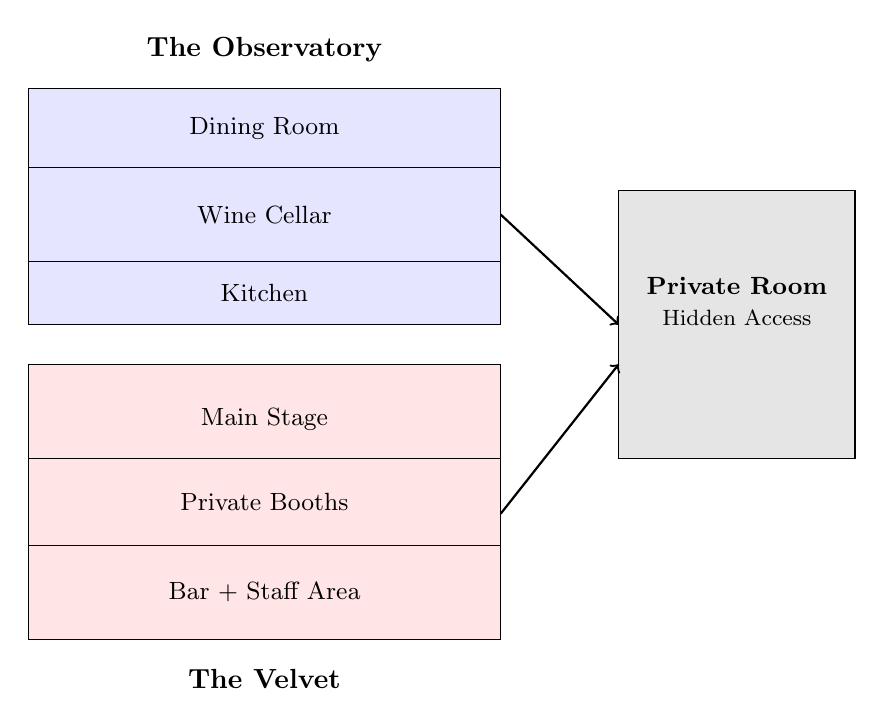
\begin{tikzpicture}[scale=1, font=\small]
  
    % === FLOOR PLAN ===
  
    % The Observatory — 1st Floor Layout
    \draw[fill=blue!10] (0,4) rectangle (6,7); % Restaurant
    \node[font=\bfseries] at (3.0, 7.5) {The Observatory};
    \draw (0,6) -- (6,6); % Divider line
    \node at (3,6.5) {Dining Room};
    \draw (0,4.8) -- (6,4.8);
    \node at (3,5.4) {Wine Cellar};
    \node at (3,4.4) {Kitchen};
  
    % The Velvet — Basement Layout
    \draw[fill=red!10] (0,0) rectangle (6,3.5); % Club
    \node[font=\bfseries] at (3,-0.5) {The Velvet};
    \draw (0,2.3) -- (6,2.3);
    \node at (3,2.8) {Main Stage};
    \draw (0,1.2) -- (6,1.2);
    \node at (3,1.75) {Private Booths};
    \node at (3,0.6) {Bar + Staff Area};
  
    % Shared Private Room
    \draw[fill=gray!20] (7.5,2.3) rectangle (10.5,5.7); 
    \node[align=center] at (9,4.3) {\textbf{Private Room}\\\footnotesize Hidden Access};
  
    % Entry arrows to Private Room
    \draw[->, thick] (6,5.4) -- (7.5,4.0); % From wine cellar
    \draw[->, thick] (6,1.6) -- (7.5,3.5); % From booths
  
    % === CORPORATE STRUCTURE ===
    %\node[font=\bfseries] at (15,8.5) {Corporate Ownership Structure};
  
    % Parent company
    %\draw[fill=black!5] (13,7.8) rectangle (17,8.3);
    %\node at (15,8.05) {\textbf{Orion Hospitality Group, LLC}};
  
    % Shells
    %\draw[fill=black!10] (13,6.8) rectangle (17,7.3);
    %\node at (15,7.05) {Shell LLC A — The Velvet};
  
    %\draw[fill=black!10] (13,5.6) rectangle (17,6.1);
    %\node at (15,5.85) {Shell LLC B — The Observatory};
  
    %\draw[fill=black!10] (13,4.4) rectangle (17,4.9);
    %\node at (15,4.65) {Shell LLC C — Private Room};
  
  \end{tikzpicture}
  \caption{
    Architectural floor plan of The Observatory (restaurant), The Velvet (club), and a hidden shared private 
    room — all legally separated by distinct shell LLCs but operated under a single parent entity.
  }
\end{figure}
  
\medskip 

The girls were not staff. But they were not exactly guests, either. The girls were just close 
enough to blur the line, and just far enough to keep anything that happened off the books.

The room itself was equal parts seduction and strategy. On the far side, a 
large circular bed 
slowly revolved under soft amber lights, not fast enough to draw attention, but just enough to suggest movement even when no 
one was on it. Opposite that, a narrow staircase led up to a small balcony lounge with low armchairs and a view that looked 
down over everything: the bed, the tables, and the guests. From up there, the whole scene played like theater.

Beneath the balcony sat a tastefully integrated dancer’s pole that was polished to a mirror finish.
Between the pole and the bed, a row of dark walnut tables offered just enough space for a whiskey flight.
Leather-backed chairs, matte black sugar trays, flickering votives completed the setup, and evoked a high-end coffee shop 
more than a club. It gave cover to whatever the guests chose to call the evening.


After dessert, it wasn’t uncommon for the night to 
migrate there.  Sometimes the wives joined. Sometimes they didn’t.  Sometimes 
they brought their own guests.  On the expense report, it was just a dinner.  It was just a networking event.  
It was just a hospitality line item.  But everyone understood. What happened in the private room wasn’t on the receipt.  
But it was part of the bargain.

If anything compromising happened in that room — a lapse in judgment, a moment of indulgence, a scene that didn’t belong 
in a compliance report — it wouldn’t trace back to the restaurant or the club. Not directly.

The layout made that possible. And so did the paperwork.

The private room acted like a firewall. It was where someone could have a ``business dinner'', and no one would ask questions. 
The circular bed wasn’t just for show, and the mirrored ceiling above it wasn’t an accident. 
Security staff knew where to turn the cameras, and the exit to the Velvet was marked only from the inside. 

\medskip

\begin{TechnicalSidebar}{Significance of a Shell LLC Leasing the Private Room}

  The decision to lease the private room under a shell company wasn’t just legal 
  hygiene. It was structural intent. It was a design principle long documented in the study 
  of offshore finance and covert institutional behavior (Sharman, 2010).

  \medskip

  \textbf{First, it created containment.}  
  In 2008, a private equity firm used an anonymous LLC registered in Delaware to lease a hospitality suite 
  during a high-profile energy summit. When investigative reporters later traced corruption charges back to 
  bribes exchanged in that suite, the hosting venue denied involvement. Legally, they were right. The 
  registered tenant was a firm with no employees and a PO box (Zucman, 2015; Christensen et al., 2020).  
  This strategy mirrors techniques used in offshore banking hubs like the British Virgin Islands, where 
  shell firms serve as “firewalls” in case something combusts.

  \medskip

  \textbf{Second, it enabled rebranding on demand.}  
  The same room could be pitched as a ``client engagement space'' to one audience, a ``wine reserve'' to another, 
  or simply as ``private event infrastructure'' to outside auditors. In one case noted by Scott (2009), 
  a high-end nightclub in Miami listed the space on internal blueprints as “HVAC Storage” while simultaneously 
  marketing it off-books to foreign clients for off-the-record political meetings.

  \medskip

  \textbf{Third, it operationalized deniability.}  
  During the FIFA corruption scandal, internal documents revealed that a ``hospitality coordination firm'' 
  had leased private rooms in Zurich under a holding company with no public affiliation to FIFA. 
  When prosecutors requested records, local staff truthfully responded that they had no direct access since 
  the rental entity maintained its own logs, keys, and contracts (Picciotto, 2007).

  \medskip

  \textbf{Fourth, it outsourced access control.}  
  By assigning keycard permissions, camera footage, and guest tracking to a legally distinct custodial 
  firm, organizations could mask patterns of influence. Levi and Reuter (2006) document how shell LLCs 
  in the arms trade leased seemingly innocuous conference rooms for “due diligence briefings,” 
  when in fact they were used for covert negotiations involving state-linked actors.

  \medskip

  \textbf{Finally, there was financial flexibility.}  
  In one audit flagged by OECD (2011), a management consultancy in London routed client entertainment 
  through a “branding advisory sub-entity,” allowing them to write off lavish dinners and private rooms 
  as R\&D expenses. Desai, Dyck, and Zingales (2007) note that shell firms often act as financial avatars: 
  enabling the recharacterization of costs, redirecting client charges across tax jurisdictions, and 
  dispersing liability across “plausible ledgers.”

  \medskip

  This wasn’t just about hiding misconduct.  
  It was about enabling modularity — an ability to change the story depending on the context, 
  the audience, or the regulatory regime (Harvey, 2005).  
  It allowed the same space to be elite hospitality, legal ambiguity, or strategic anonymity 
  (depending on what the moment required).

\end{TechnicalSidebar}

  
